\chapter{Analiza problemu}
\thispagestyle{chapterBeginStyle}
\label{rozdzial1}

\section{Zadanie transportowe}
Zadanie transportowe należy do grupy zadań optymalizacyjnych z ograniczeniami. Rozwiązując je staramy się przy użyciu $n$ punktów nadania 
zaspokoić zapotrzebowanie $m$ punktów odbioru w taki sposób, aby całkowity koszt transportu był minimalny. Zadanie wymaga określenia ilości 
towaru znajdującej się w każdym z punktów nadania, oraz zapotrzebowania na towar w każdym z punktów odbioru. Dodatkowo musimy określić 
koszt transportu pomiędzy każdym punktem nadania i każdym punktem odbioru. Klasyczne zadanie transportowe ogranicza się do transportu 
tylko jednego towaru, dzięki czemu punkty odbioru mogą być zaopatrywane przez jeden lub więcej punktów nadania.

Zadanie transportowe nazywamy zbilansowanym, jeśli całkowita podaż towaru jest równa całkowitemu popytowi. W przeciwnym wypadku 
zadanie jest niezbilansowane. Rozwiązywanie zadania niezbilansowanego polega na sprowadzeniu go do zadania zbilansowanego, poprzez 
dodanie fikcyjnego dostawcy(w przypadku większego popytu), lub fikcyjnego odbiorcy(w przypadku większej podaży). Wartość kosztu dostawy 
między fikcyjnym dostawcą a odbiorcami, lub między dostawcami a fikcyjnym odbiorcą najczęściej ustalany jest jako zerowy.

Załóżmy, że mamy $n$ punktów nadania i $m$ punktów odbioru. Początkowa ilość towaru w $i$-tym punkcie nadania jest równa $supply(i)$, 
a początkowe zapotrzebowanie w $j$-tym punkcie odbioru jest równe $demand(j)$. Jeśli $x_{ij}$ jest ilością towaru dostarczanego przez 
$i$-ty punkt nadania do $j$-tego punktu odbioru, to zbilansowane zadanie transportowe możemy zdefiniować w następujący sposób:

$$min \sum_{i=1}^{n} \sum_{j=1}^{m} f_{ij}(x_{ij})$$

Przy spełnionych ograniczeniach:
$$\sum_{j=1}^{m} x_{ij} = supply(i), \text{ dla } i = 1, 2, \dots, n$$
$$\sum_{i=1}^{n} x_{ij} = demand(j), \text{ dla } j = 1, 2, \dots, m$$
$$x_{ij} \ge 0, \text{ dla } i = 1, 2, \dots, n \text{ i } j = 1, 2, \dots, m$$

Pierwszy zestaw ograniczeń mówi o tym, że całkowita ilość towaru transportowana z pojedynczego punktu nadania musi być równa jego początkowej 
ilości znajdującej się w tym punkcie. Z kolei drugi zestaw mówi o tym, że całkowita ilość towaru transportowana do pojedynczego punktu odbioru 
musi być równa jego początkowemu zapotrzebowaniu. W przypadku zadania niezbilansowanego równości w dwóch pierwszych zestawach ograniczeń należy 
zmienić na odpowiednie nierówności. Zadanie jest liniowe, jeśli koszt transportu między punktami nadania i odbioru jest wprost proporcjonalny 
do ilości transportowanego towaru, tzn. jeśli $f_{ij}(x_{ij}) = cost_{ij} x_{ij}$, gdzie $cost_{ij}$ jest jednostkowym kosztem transportu 
między $i$-tym punktem nadania, a $j$-tym punktem odbioru.

\subsection{Wersja liniowa}
Zadanie transportowe w wersji liniowej należy do problemów programowania liniowego, a więc można rozwiązać je przy pomocy algorytmu sympleks.
$$[...TODO...]$$

\subsection{Wersja nieliniowa}
O ile liniowa wersja zadania jest stosunkowo łatwa w rozwiązaniu, o tyle dla wersji nieliniowej nie ma ogólnej metody rozwiązywania. Należy 
ono do problemów z kategorii NP-trudnych [TODO - znalezc publikacje]. Do jego rozwiązania używa się różnych algorytmów wyznaczających 
rozwiązania przybliżone, takich jak algorytmy metaheurystyczne.



\section{Klasyczne rozwiązania}


\section{Algorytmy metaheurystyczne}
Algorytmy metaheurystyczne znajdują zastosowanie szczególnie przy rozwiązywaniu nieliniowego zadania transportowego, ponieważ w tym przypadku 
nie są znane algorytmy, które wyznaczają dokładne rozwiązanie w akceptowalnym czasie. 

[TODO: dopisac]

\subsection{Algorytmy ewolucyjne}
Algorytmy ewolucyjne stanowią podzbiór algorytmów metaheurystycznych. Sposób ich działania jest inspirowany przez zjawisko ewolucji występujące 
w naturze. Na początku działania algorytmu generowana jest w sposób losowy populacja startowa. Procedurę generowania pojedynczego osobnika lub 
całej populacji nazywać będziemy \textbf{inicjalizacją}. Następnie na przestrzeni pokoleń(iteracji algorytmu) 
populacja ewoluuje generując coraz lepsze rozwiązania. W każdej iteracji pewna część osobników zostaje wybrana do reprodukcji. Procedurę wyboru 
rodziców do reprodukcji nazywać będziemy \textbf{selekcją}. Wybrane osobniki krzyżujemy między sobą, tworząc w ten sposób nowe, 
posiadające cechy wybranych wczesniej rodziców. Następnie losowo wybrane osobniki ulegają mutacji. 
Ostatecznie z otrzymanych osobników tworzona jest nowa populacja, która będzie stanowić bazę dla kolejnej iteracji algorytmu. Algorytm kończy 
działanie w momencie kiedy zostanie spełniony warunek końcowy, którym może być np. wygenerowanie wystarczająco dobrego rozwiązania lub 
przejście określonej liczby iteracji.

\begin{pseudokod}
\caption{Ogólny schemat działania algorytmu ewolucyjnego}
\label{alg_ewo}
    $P(t)$: Populacja w t-tej iteracji algorytmu\;
    $O(t)$: Populacja dzieci w t-tej iteracji algorytmu\;

    $t \gets 0$\;
    inicjalizacja $P(t)$\;
    \While{Warunek końcowy nie został spełniony} {
        $parents \gets$ selekcja z $P(t)$\;
        $O(t+1) \gets$ zastosuj operator krzyżowania na $parents$\;
        $O(t+1) \gets$ zastosuj operator mutacji na $O(t+1)$\;
        $P(t+1) \gets$ wybierz osobniki do następnej generacji z $O(t+1)$\;
        $t \gets t+1$\;
    }
    \Return{najlepszy osobnik z $P(t)$}\;
\end{pseudokod}

\begin{figure}[h]
    \centering        
    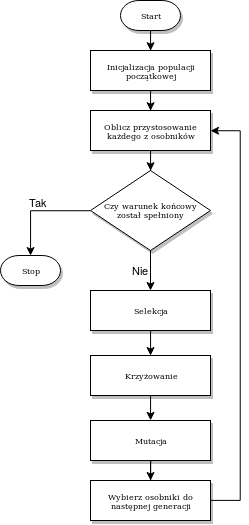
\includegraphics[width=0.4\textwidth]{img/alg_ewo_szkic.png}
    \caption{Ogólny schemat działania algorytmu ewolucyjnego}
    \label{alg_ewo_img}
\end{figure}

Projektowanie algorytmu ewolucyjnego możemy podzielić na kilka oddzielnych części, są to: 
\begin{itemize}
    \item Reprezentacja - określa sposób zakodowania rozwiązania w chromosomie. Wybór reprezentacji chromosomu jest bardzo ważnym etapem 
    projektowania algorytmu. Odpowiednia reprezentacja może w znacznym stopniu wpłynąć na szybkość i jakość rozwiązań znajdowanych przez 
    algorytm, ponieważ to ona w dużej mierze określa sposób w jaki przeszukiwana będzie przestrzeń rozwiązań zadania. 
    Jako reprezentacje bardzo często stosowane są wektory lub macierze genów, gdzie gen może być pojedynczą liczbą całkowitą lub rzeczywistą. 
    Oczywiście jako sposób reprezentacji rozwiązania możemy wybrać dowolną strukturę danych, należy jednak pamiętać, że zdefiniowane później 
    operacje mutacji i krzyżowania muszą być dostosowane do wybranej struktury.
    
    \item Funkcja oceny - określa stopień przystosowania danego osobnika. Bardzo często funkcja oceny jest równoważna funkcji celu, którą 
    nasz algorytm ma minimalizować/maksymalizować, nie jest to jednak regułą. 

    \item Operator krzyżowania - jest jednym z operatorów używanych do generowania kolejnego pokolenia w algorytmach ewolucyjnych. Z założenia 
    przyjmuje on jako argumenty dwa lub więcej rozwiązań(rodziców) i generuje na ich podstawie nowe(dzieci), które łączą w sobie cechy rodziców. 
    [TODO: przykład]

    \item Operator mutacji - jest drugim z operatorów używanych do generowania następnych pokoleń w algorytmach ewolucyjnych. Jego celem jest 
    poszerzene obszaru przeszukiwanych rozwiązań. Ten operator powinien wprowadzać minimalną zmianę w rozwiązaniu, co zapobiega zbyt szybkiej 
    zbieżności algorytmu i pozwala na wprowadzenie dodatkowej różnorodności w populacji. Należy pamiętać o tym, że wprowadzana zmiana nie może 
    być za duża, bo może to prowadzić do odwrotnego rezultatu, czyli zamiast różnicować rozwiązania nasz operator może je niszczyć.
    [TODO: przykład]

    \item Selekcja - określa sposób wyboru rodziców na których użyjemy operatora krzyżowania. Istnieje wiele opisanych metod selekcji\cite{SELECTION-METHODS} 
    takich jak np. metoda koła ruletki czy metoda rankingowa. Przy tworzeniu procedury selekcji należy pamiętać 
    o tym, że rozwiązania lepiej przystosowane powinny mieć większe szanse na zostanie rodzicami dla kolejnego pokolenia. Zapewnia to większe 
    szanse na wygenerowanie lepszych dzieci do następnej generacji.
    [TODO: przyklad]

    \item Wybór następnego pokolenia - ostateczny krok algorytmu, w którym wybieramy które osobniki wejdą w skład populacji początkowej w 
    kolejnej iteracji algorytmu. Podstawową składową tej populacji powinny być oczywiście osobniki wygenerowane za pomącą krzyżowania. Często 
    stosowaną praktyką jest również przepisywanie części najlepszych rozwiązań oraz kilku losowo wybranych z poprzedniego pokolenia. 

\end{itemize}